% ==============================================================================
% Section 5: Model Description
% ==============================================================================

\section{Model Description}
\label{sec:model}

This section describes the structure and mechanics of the SSWD-EvoEpi
agent-based model.  Readers interested primarily in conservation
implications may proceed to the Discussion (Section~\ref{sec:discussion});
what follows is intended for those who wish to understand how the
forecasts were generated.

% --------------------------------------------------------------------------
\subsection{Agent-Based Framework}
\label{sec:abm_framework}

The model simulates individual \textit{Pycnopodia helianthoides} across
\textbf{896 coastal sites} spanning the species' entire historical range,
from the western Aleutian Islands (52.5\textdegree N) to central Baja
California (28.5\textdegree N).  Sites are grouped into 18 geographic
regions corresponding to major oceanographic and biogeographic boundaries
(e.g., Prince William Sound, Salish Sea, Oregon coast, Channel Islands).
Each site supports up to $K = 5{,}000$ individuals, yielding a theoretical
coast-wide carrying capacity of approximately 4.5~million sea stars.

% --- Figure: Network Map (from progress report) ---
\begin{figure}[!htbp]
    \centering
    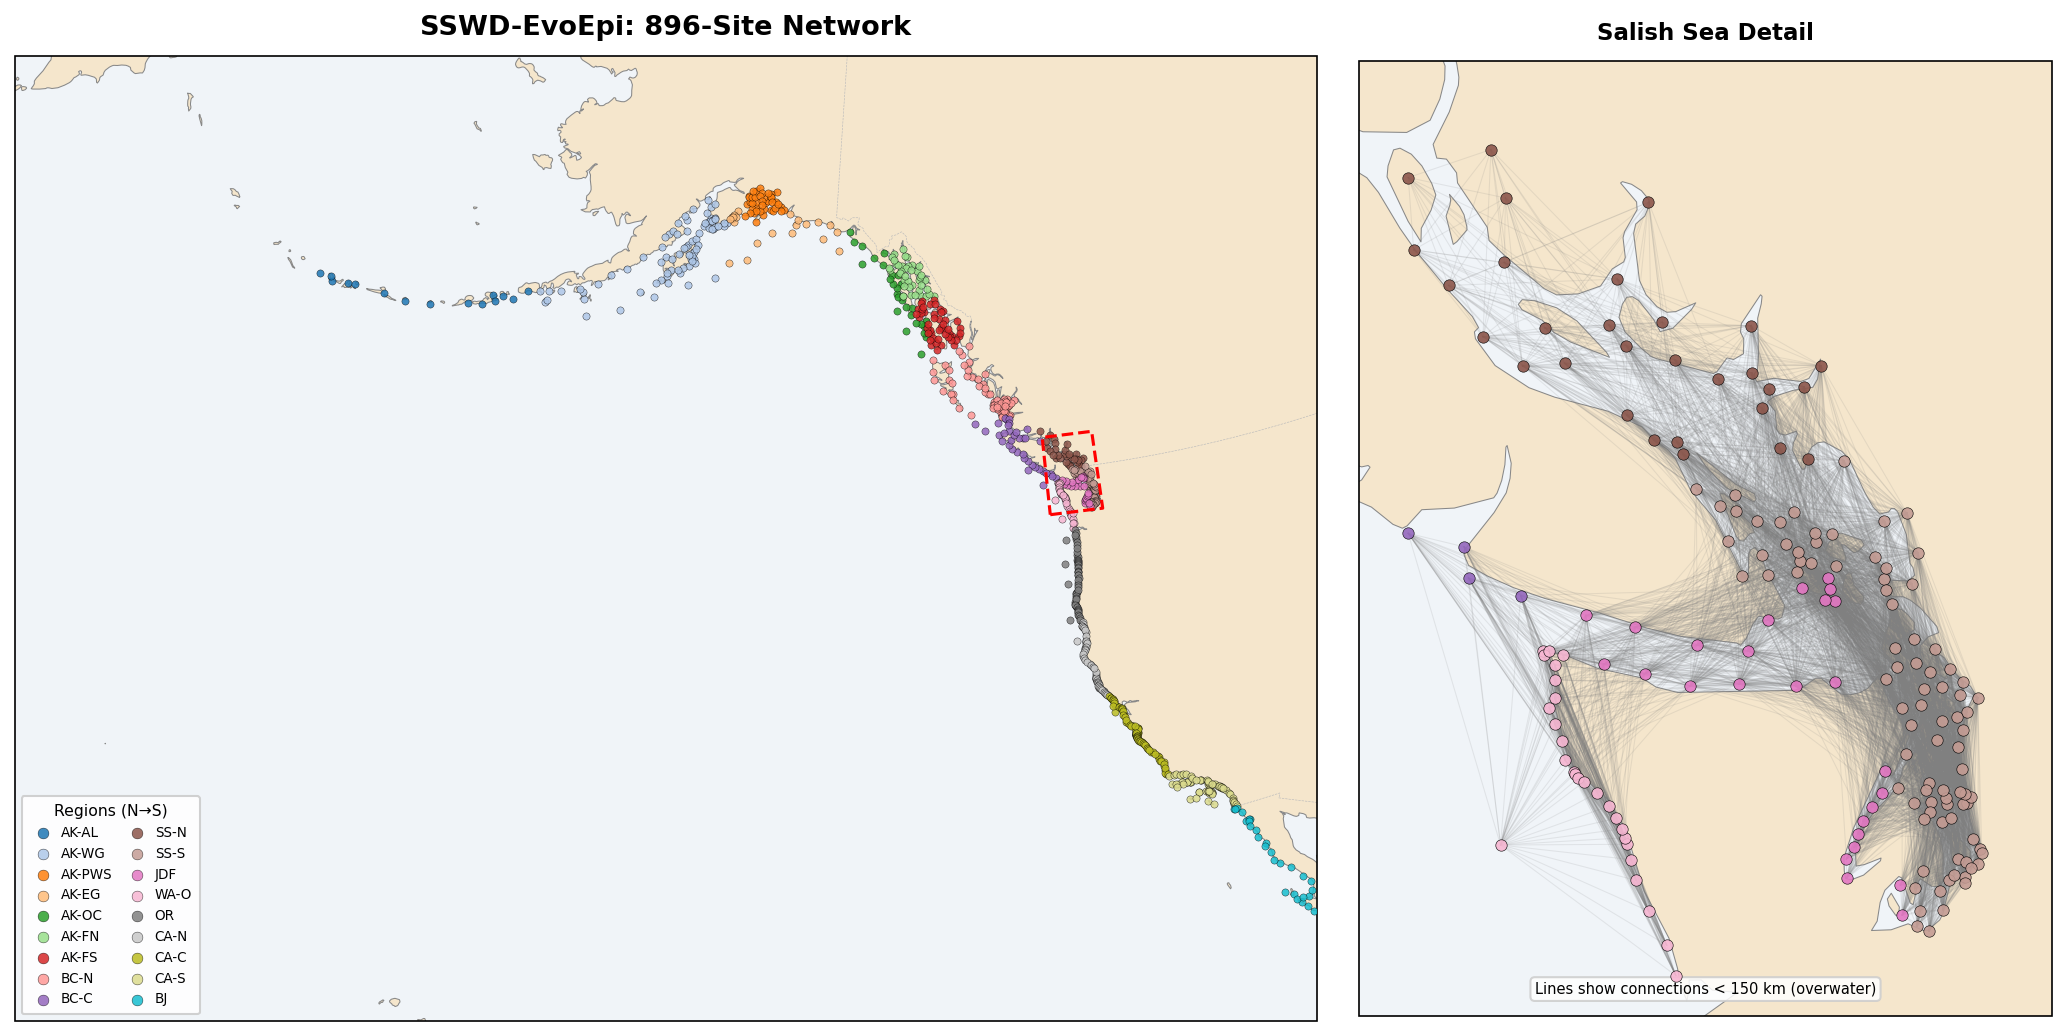
\includegraphics[width=0.85\textwidth]{figures/fig_network_map.png}
    \caption{The 896-site spatial network spanning Alaska (Aleutian Islands) to Baja California, colored by 18 geographic regions. Sites are connected by larval dispersal ($D_L = 400$~km exponential decay) and waterborne pathogen transport ($D_P = 300$~km) kernels. The inset panel zooms into the Salish Sea, where gray connectivity lines illustrate the dense local network structure through which larvae and pathogen disperse.}
    \label{fig:network_map}
\end{figure}

The simulation operates in \textbf{daily timesteps} from 2012 through 2050.
Each simulated day steps through disease transmission, individual survival,
growth, and---during the spawning season---reproduction and larval dispersal.

Each individual sea star is represented as a distinct agent carrying the
following attributes:
\begin{itemize}
  \item \textbf{Position} ($x, y$ in meters) and \textbf{heading}
        (direction of travel) within its home site;
  \item \textbf{Body size} (arm-tip diameter in mm, growing via von
        Bertalanffy dynamics toward $L_\infty = 1{,}000$\,mm);
  \item \textbf{Age} and \textbf{sex};
  \item \textbf{Disease state} (susceptible, exposed, pre-symptomatic,
        symptomatic, or dead);
  \item \textbf{51 genetic loci} governing three heritable defense traits
        (Section~\ref{sec:host_genetics}).
\end{itemize}

Individuals move within sites via a \textbf{correlated random walk} at a
base speed of 0.5\,m/min \citep{hodin2021}, resolved in 24 hourly substeps
per day.  Symptomatic individuals slow to 10\% of normal speed; dead
individuals do not move.  Movement matters because disease transmission is
\textbf{spatially explicit}: a 20\,m grid within each site tracks local
pathogen concentrations, so stars near clusters of infected individuals
experience higher exposure than those farther away.

\paragraph{Temperature forcing.}
All scenarios are driven by \textbf{observed sea surface temperature (SST)}
from the NOAA Optimum Interpolation SST v2.1 dataset for 2012--2025,
bilinearly interpolated to each of the 896 model sites.  For the projection
window (2026--2050), SSTs are generated via a delta method applied to CMIP6
general circulation models (Section~\ref{sec:sst_projections}).  Real
climate events---including the 2013--2016 marine heatwave, El~Ni\~no, and
La~Ni\~na cycles---are thus automatically incorporated during the
historical period.

% --------------------------------------------------------------------------
\subsection{Disease Mechanics}
\label{sec:disease}

The disease module simulates the dynamics of \textit{Vibrio pectenicida},
recently confirmed as the etiological agent of SSWD through fulfillment of
Koch's postulates \citep{prentice2025}.  Its structure rests on two
biological pillars: a modified SEIR compartmental model within individual
hosts, and the VBNC (viable but non-culturable) dormancy state that couples
pathogen activity to water temperature.

\paragraph{Within-host progression.}
Each individual follows a five-stage disease progression:
\begin{center}
S $\to$ E $\to$ I$_1$ (pre-symptomatic) $\to$ I$_2$ (symptomatic)
  $\to$ Dead
\end{center}
Transition rates between compartments are Arrhenius-scaled (i.e., exponentially increasing with temperature) to local SST,
meaning disease progresses faster in warmer water.  At a reference
temperature of 20\textdegree C, the mean time from exposure to death is
approximately 6~days ($\mu_{EI_1} = 0.233$/d, $\mu_{I_1 I_2} = 0.434$/d,
$\mu_{I_2 D} = 0.563$/d).  Pre-symptomatic individuals shed pathogen at a
rate of $\sigma_1 = 5.0$ units/day; symptomatic individuals shed ten-fold
more ($\sigma_2 = 50.0$).  Dying stars release a burst of $\sigma_D = 15.0$
units.  Recovered individuals return to susceptible status---echinoderms
lack adaptive immunity, so reinfection is possible \citep{prentice2025}.

\paragraph{The VBNC state.}
\textit{Vibrio} species enter a dormant VBNC state in cold water
\citep{liu2019}.  We model this as a sigmoid transition centered at
$T_\mathrm{vbnc} = 12$\textdegree C (steepness $k = 2.0$): at
14\textdegree C the pathogen is ${\sim}$98\% active, at 12\textdegree C
it is 50\% active, and at 10\textdegree C only ${\sim}$2\% remains active.
A biophysical floor of $T_\mathrm{vbnc,min} = 9$\textdegree C prevents any
evolutionary adaptation below this temperature (Section~\ref{sec:pathogen_evo}).

This mechanism has profound geographic consequences.  In southern California,
where SST routinely exceeds 12\textdegree C, the pathogen is active
year-round and disease pressure is relentless.  In Alaska, where SST only
briefly exceeds the threshold in summer, stars receive a seasonal reprieve
during the cold months---but the pathogen persists in dormancy, ready to
reactivate each warm season.

\paragraph{Environmental pathogen pool.}
Each site maintains a dynamic environmental reservoir of \textit{Vibrio}.
The pool grows as infected individuals shed pathogen (fraction
$\alpha_\mathrm{env} = 0.18$ enters the persistent pool) and decays
naturally ($\delta_\mathrm{env} = 0.02$/day, half-life $\approx$35~days).
A susceptible star's daily infection probability follows Michaelis--Menten
kinetics with a half-saturation constant $K_\mathrm{half} = 800{,}000$,
modified by the individual's resistance trait, body size, and local VBNC
activation.  This density-dependent mechanism creates a positive feedback
loop: more infected individuals shed more pathogen, raising the
environmental pool, which drives further infections.  At high host density,
this feedback can collapse a site within weeks; at low density, the same
parameters produce modest mortality because the pool never builds to
saturating levels.

% --- Figure: Within-site Disease (from progress report) ---
\begin{figure}[!htbp]
    \centering
    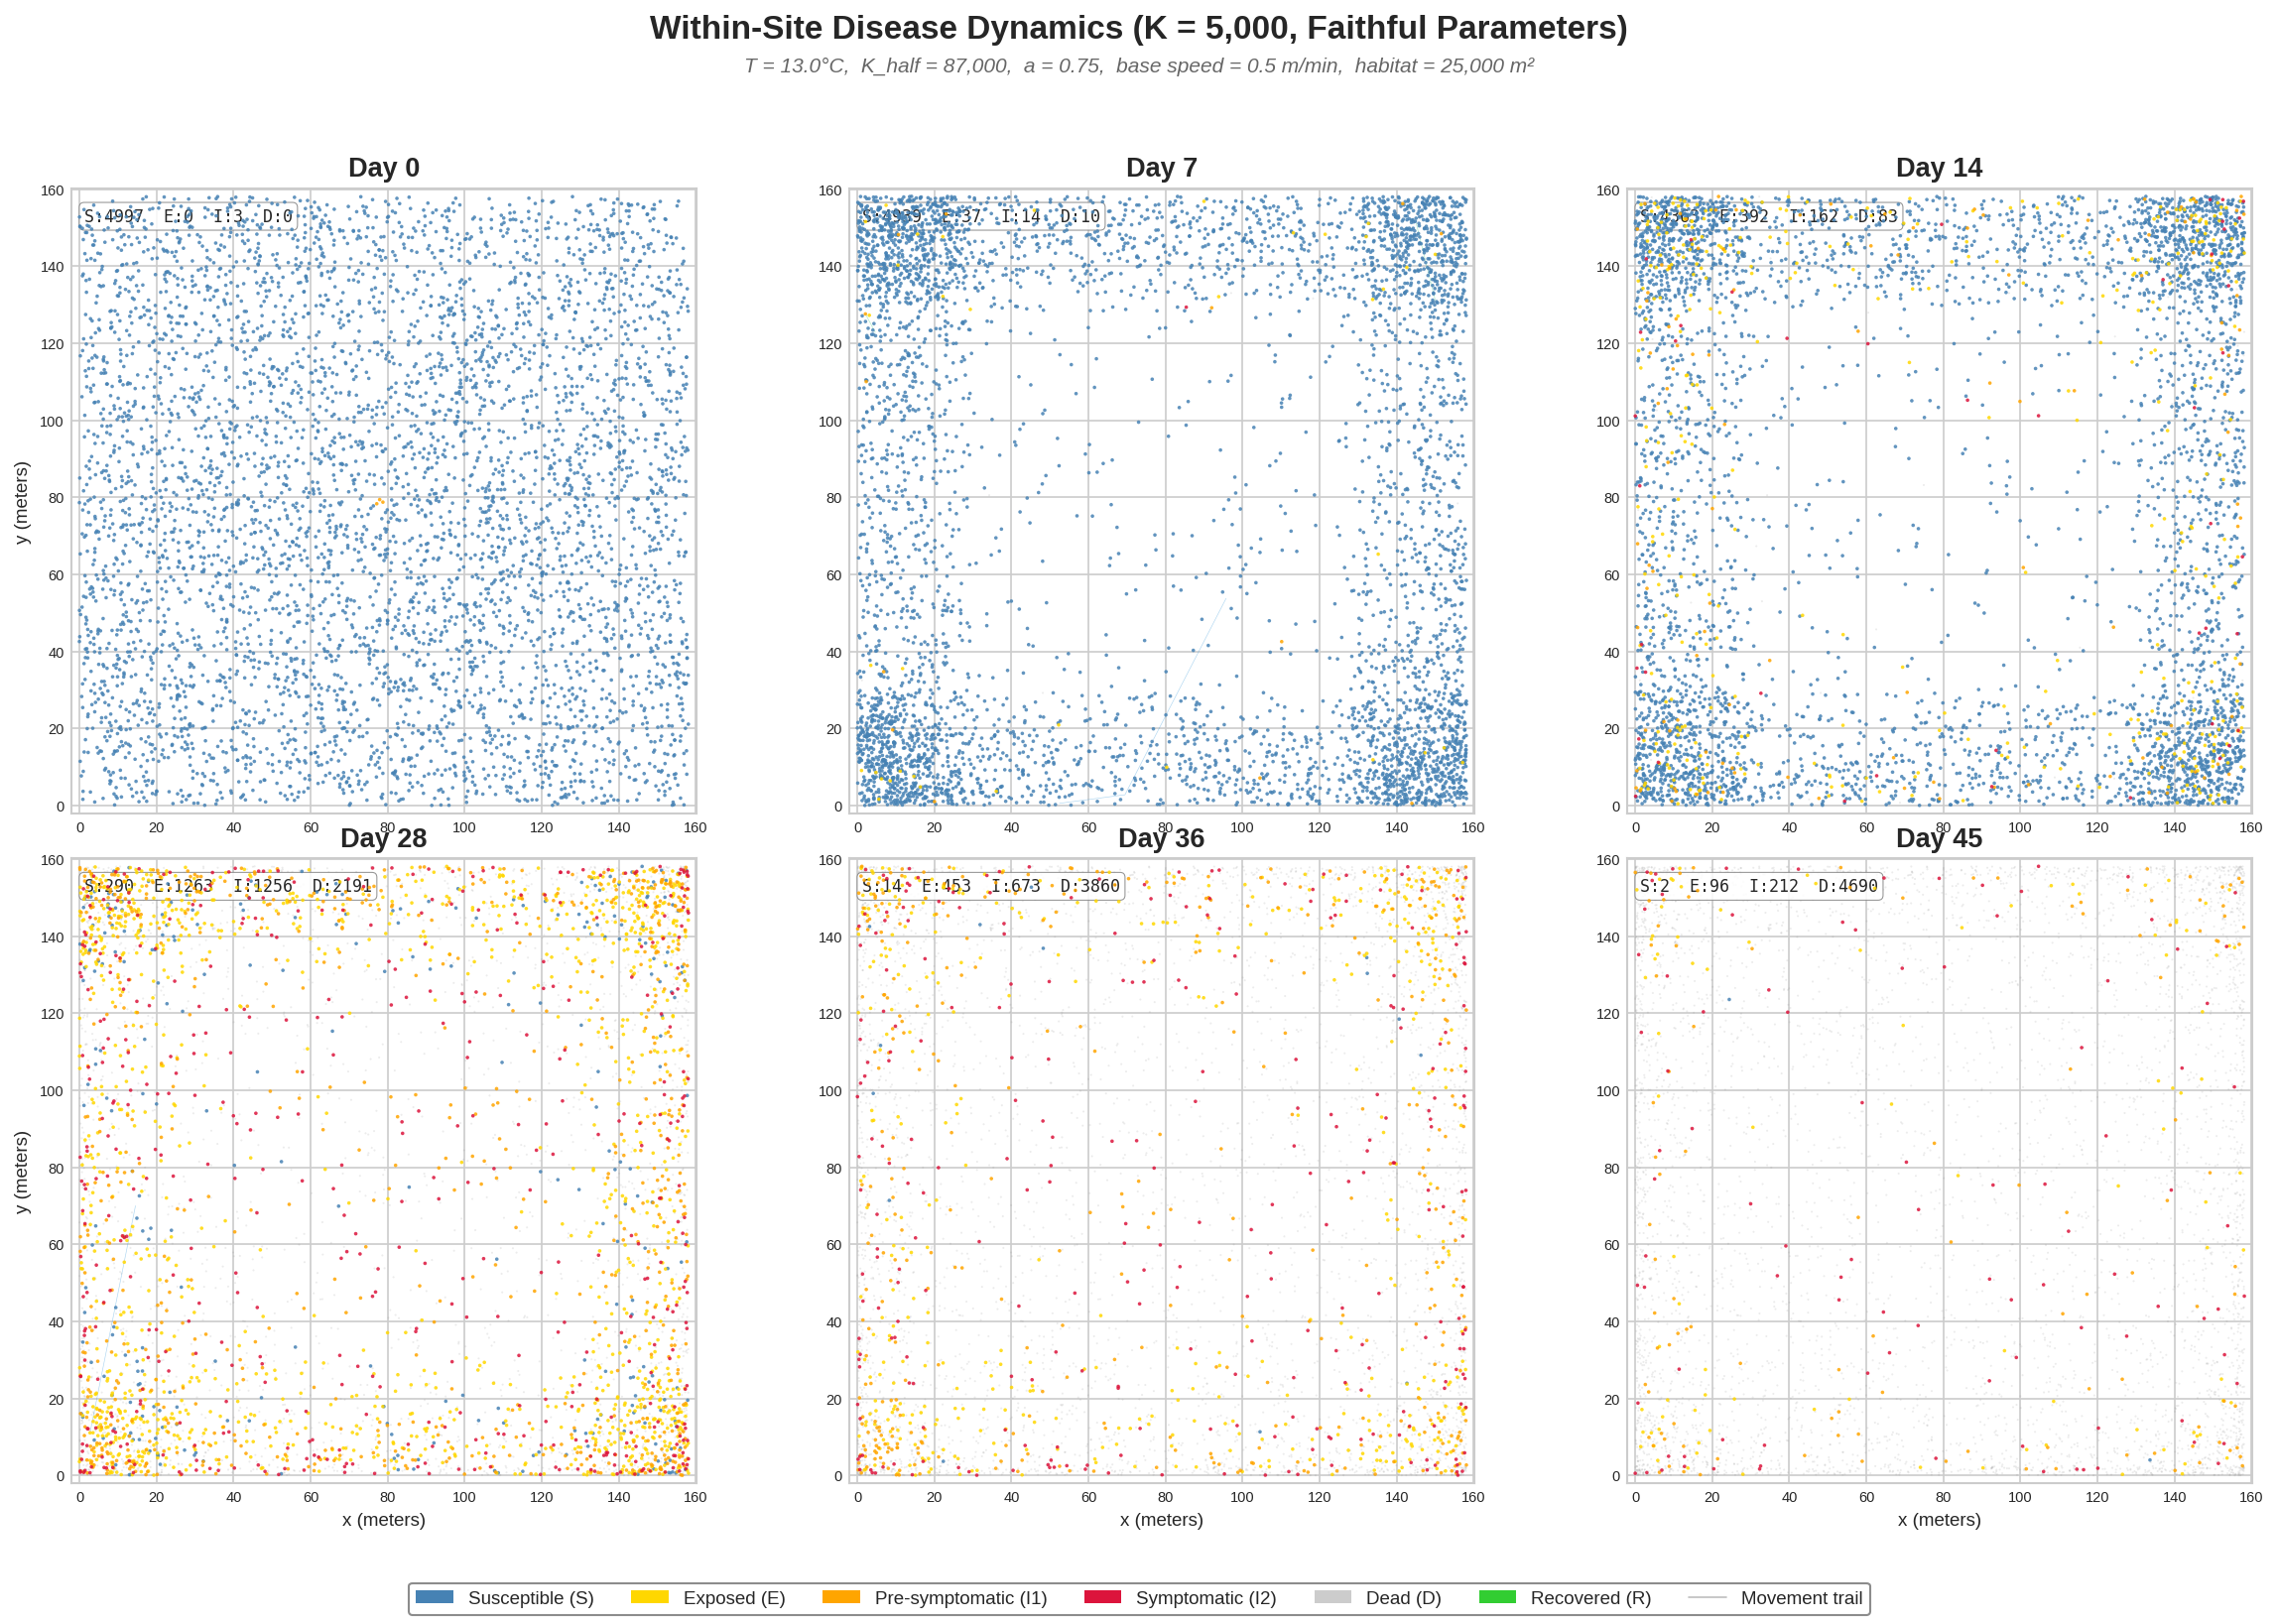
\includegraphics[width=0.95\textwidth]{figures/fig_within_site_disease.png}
    \caption{Simulated within-site disease dynamics using the model's actual spatial transmission mechanics ($K = 5{,}000$ individuals, 158$\times$158~m habitat, $T = 13$\textdegree C). Disease begins with 3 pre-symptomatic individuals (Day~0). By Day~14, exposed (gold) and infected (orange/red) individuals are spreading through spatial proximity effects. Day~28 is peak infection (1,256 active infected). By Day~45, 93.8\% of the population is dead. Zero individuals recovered, consistent with the very low initial recovery ability ($\bar{c} = 0.02$). The rapidity of collapse at high density contrasts with only $\sim$12\% mortality at low density, illustrating the density-dependent positive feedback in pathogen dynamics.}
    \label{fig:within_site_disease}
\end{figure}

\paragraph{Wavefront propagation.}
Consistent with observational records, disease originates from five sites
in the Channel Islands (southern California) in mid-2013 and spreads as a
northward wave.  Three mechanisms interact to produce the wavefront:
(1)~thermal activation requires SST to exceed $T_\mathrm{vbnc}$ before the
pathogen can establish locally, so southern sites ignite first;
(2)~a cumulative dose threshold of 1{,}000 units must be reached before
local outbreak onset, creating a realistic lag between first exposure and
epizootic; and (3)~waterborne pathogen disperses between connected sites
via an exponential decay kernel ($D_P = 300$\,km characteristic distance),
allowing the disease front to propagate along the coast.

% --- Figure: Disease Wavefront Snapshots (from progress report) ---
\begin{figure}[!htbp]
    \centering
    
\includegraphics[width=0.95\textwidth]{figures/fig_disease_snapshots.png}
    \caption{Four snapshots of the range-wide disease simulation. \textbf{Top left:} Pre-disease (2012), all populations near carrying capacity. \textbf{Top right:} Peak crash (2014--2015), disease spreading northward from southern California. \textbf{Bottom left:} Mid-simulation (2016--2017), partial recovery in Alaska driven by seasonal pathogen dormancy. \textbf{Bottom right:} Final state (2024), showing the persistent north--south gradient in population survival.}
    \label{fig:disease_snapshots}
\end{figure}

% --------------------------------------------------------------------------
\subsection{Host Genetics and Evolution}
\label{sec:host_genetics}

Each individual carries \textbf{51 diploid genetic loci} divided equally
among three heritable defense traits, inspired by genome-wide association study (GWAS) results from the
congener \textit{Pisaster ochraceus} \citep{schiebelhut2018}---the only
Pacific asteroid for which disease-associated genomic data currently exist.
No equivalent GWAS has yet been conducted for \textit{Pycnopodia}.

\begin{description}
  \item[Resistance ($r$, 17 loci):] Scales the individual's infection
    hazard rate by $(1-r)$.  A star with $r = 0.30$ experiences a 30\%
    reduction in its instantaneous infection risk per unit pathogen
    exposure.  Think of it as an \textit{armor rating}.

  \item[Tolerance ($t$, 17 loci):] Extends survival during symptomatic
    (I$_2$) infection, reducing the rate of progression to death.  A
    tolerant star lives longer while infected, buying time for possible
    clearance.

  \item[Recovery ($c$, 17 loci):] Scales the daily probability of
    clearing the pathogen.  Effective daily clearance is
    $\rho_\mathrm{rec} \times c$, where $\rho_\mathrm{rec} = 0.05$.
    Cleared individuals return to susceptible status (R$\to$S; no
    adaptive immunity in echinoderms).
\end{description}

Locus effect sizes follow an exponential distribution (a few loci of large
effect, many of small effect), and traits are computed as additive sums
across their respective loci.  Initial trait values---$r_0 = 0.15$,
$t_0 = 0.10$, $c_0 = 0.02$---reflect a largely na\"ive population prior to
the 2013 outbreak.  At $c_0 = 0.02$, the effective daily clearance rate is
just 0.1\%, meaning recovery from active infection is extremely rare.

\paragraph{Natural selection.}
Selection operates straightforwardly: individuals that survive disease
disproportionately carry favorable alleles at defense loci.  When survivors
reproduce, they pass those alleles to offspring.  Over generations, mean
defense trait values increase.  By 2050, resistance in hard-hit southern
populations rises from 0.15 to approximately 0.43, while
less-affected northern populations evolve more slowly ($r \approx 0.20$--0.25).
However, even $r = 0.45$ still leaves more than half of the pathogen force
unblocked---evolution is real but not a rescue.

A critical secondary effect is \textbf{genetic diversity loss}.  Populations
that crash to near-zero lose most of their standing genetic variation.
The additive genetic variance ($V_A$) for resistance in southern
California---the raw material for future adaptation---collapses from
0.026 to 0.003, an 88\% reduction.  The populations most in need of
continued evolution have the least capacity for it.

% --------------------------------------------------------------------------
\subsection{Pathogen Community Evolution}
\label{sec:pathogen_evo_model}

Rather than tracking individual bacterial strains, the model treats the
pathogen community at each site as the evolutionary unit---an aggregate
whose properties shift in response to local selection pressures.  Each
community has two evolving traits:

\paragraph{Thermal activation threshold ($T_\mathrm{vbnc}$).}
The temperature midpoint for the VBNC sigmoid drifts downward at cold-water
sites where there is sustained selection for cold-tolerant strains.  In
Alaska, the community threshold evolves from 12\textdegree C to approximately
9.0--9.4\textdegree C over the simulation, extending the active disease
season by several weeks.  At warm southern sites, where the pathogen is
already active year-round, the threshold barely changes---there is no
selection pressure for further cold adaptation.  Evolution of this trait is
bounded by a hard biophysical floor at 9\textdegree C.

\paragraph{Local virulence ($v_\mathrm{local}$).}
Virulence evolves according to the classic virulence--transmission trade-off
\citep{anderson1982}.  A more virulent pathogen kills hosts faster,
generating larger pathogen bursts, but also terminates shedding sooner.  The
optimal strategy depends on local conditions: in warm, high-density
environments, high virulence is favored (quick kill, many available hosts);
in cold, sparse environments, lower virulence is favored (host kept alive
longer, maximizing total transmission during a brief warm window).  Each
site's community drifts toward a local optimum, producing a latitudinal
gradient from $v \approx 0.08$ in Alaska to $v \approx 0.35$ in Baja
California.

The combination of thermal adaptation and virulence evolution creates
distinct pathogen strategies across the range: northern communities are
\textit{more cold-tolerant but less virulent}, while southern communities
are \textit{already warm-adapted but highly aggressive}.

% --------------------------------------------------------------------------
\subsection{Reproduction and Dispersal}
\label{sec:reproduction}

\paragraph{Broadcast spawning.}
Sunflower stars reproduce via broadcast spawning, releasing eggs and sperm
into the water column.  Spawning timing follows a latitude-dependent
schedule (peak spawning day $= 50 + 3 \times [\text{latitude} - 48.5^{\circ}]$),
with the season running from November through March \citep{hodin2021}.
Alaskan populations spawn later (mid-March) than Californian populations
(mid-January).

\paragraph{Sweepstakes reproductive success.}
Reproductive output follows the Hedgecock sweepstakes hypothesis
\citep{hedgecock2011}: in any spawning event, a small fraction of adults
contribute disproportionately to the next generation.  We implement this
as a Pareto-weighted random lottery (shape $\alpha = 1.35$), where each
reproductive adult receives a random weight from a heavy-tailed distribution.
This amplifies genetic drift, reduces effective population size ($N_e$)
well below the census count, and means that recovery genetics depend
heavily on \textit{which} individuals happen to win the reproductive
lottery---not just how many survive.

\paragraph{Larval dispersal.}
Larvae disperse between connected sites via an exponential decay kernel
with characteristic distance $D_L = 400$\,km.  Rather than modeling
hydrodynamic transport, we use a simplified connectivity scheme weighted by
overwater distance between sites and modified by coastal geometry.  Settler
survival is 0.1\%---consistent with the extremely high larval mortality
typical of marine invertebrates.

\paragraph{Allee effects.}
The model incorporates a \textbf{double Allee effect} at depleted sites.
First, fertilization success depends on local adult density via
Lundquist--Botsford kinetics ($F(\rho) = 1 - e^{-\gamma \rho_\mathrm{eff}}$,
$\gamma = 4.5$\,m$^2$): at low density, eggs fail to encounter sperm.
Second, larval settlement success follows a Michaelis--Menten curve from
20\% (substrate cues only) to 100\% (full adult chemical cues), so sites
with few adults are difficult for larvae to recolonize.  Together, these
mechanisms create an extinction vortex at very low densities---directly
relevant to reintroduction planning, where release cohorts must be large
enough to overcome both thresholds.

Pre-spawning aggregation behavior partially mitigates the fertilization
Allee effect: for 14 days before and after spawning, individuals' movement
is biased toward nearby conspecifics within a 100\,m detection range,
raising effective local density in clumps.

\paragraph{The enclosedness metric.}
A novel feature of the model is an algorithmic measure of each site's
geographic enclosure based on surrounding coastline geometry.  Sites deep
within fjords or inland seas score high; exposed outer-coast headlands score
low.  Enclosedness controls an inherent trade-off:
\begin{itemize}
  \item \textbf{Larval retention} increases at enclosed sites (good for
    recovery---local reproduction contributes more to local recruitment).
  \item \textbf{Pathogen retention} also increases (bad for disease
    escape---the same physical barriers that trap larvae trap waterborne
    \textit{Vibrio}).
\end{itemize}
Per-site flushing rates are computed as $\varphi = f(\text{enclosedness},\;
n_\mathrm{conn} = 0.3)$, with the nonlinear exponent $n_\mathrm{conn}$
calibrated to balance these opposing effects.  Self-recruitment fractions
interpolate continuously from 2\% (open coast) to 70\% (deep fjord).

% --------------------------------------------------------------------------
\subsection{Calibration Summary}
\label{sec:calibration}

The production model (designated \textbf{W154}) was selected after 154
iterative calibration rounds, each testing different parameter combinations
against empirical data.  Two classes of targets were used:

\begin{description}
  \item[Disease arrival timing:] 17 regional targets for when SSWD was first
    documented, from the Channel Islands (mid-2013) to Alaska (2015--2016),
    drawn from published case reports and monitoring programs.
  \item[Recovery fractions:] Fractional population recovery at each region by
    $\sim$2024.  The initial crash magnitude is well constrained by published
    survey data \citep{gravem2021, gehman2025}, but no consolidated range-wide
    assessment of current \textit{Pycnopodia} population status exists.
    Recovery targets were therefore estimated through expert consultation with
    field researchers across the species' range, synthesizing unpublished dive
    survey data and researcher experience into order-of-magnitude targets
    spanning 50\% (Prince William Sound, substantial cold-water recovery) to
    0.1\% (northern California, near-extirpation).  See
    Appendix~\ref{sec:appendix_targets} for details.
\end{description}

Overall fit is quantified by the \textbf{log-RMSE} (root-mean-square error
of log-transformed recovery fractions), which weights relative errors equally
across the four-order-of-magnitude range of targets.  W154 achieves a
three-seed mean RMSE of \textbf{0.504} (best single seed: 0.479).

Key calibrated parameters:
\begin{center}
\small
\begin{tabular}{llp{8cm}}
\toprule
\textbf{Parameter} & \textbf{Value} & \textbf{Interpretation} \\
\midrule
$K$ & 5{,}000 & Per-site carrying capacity \\
$K_\mathrm{half}$ & 800{,}000 & Environmental pathogen for 50\% infection rate \\
$\alpha_\mathrm{env}$ & 0.18 & Fraction of host shedding entering persistent pool \\
$\delta_\mathrm{env}$ & 0.02/d & Environmental pathogen decay rate \\
$n_\mathrm{conn}$ & 0.3 & Enclosedness-to-flushing nonlinearity \\
$D_P$ & 300\,km & Waterborne pathogen dispersal distance \\
$D_L$ & 400\,km & Larval dispersal distance \\
\bottomrule
\end{tabular}
\end{center}

\paragraph{Known limitation.}
The model's main calibration challenge is Alaska.  W154 produces 2--7\%
recovery in Prince William Sound and Fairweather against 50\% survey-based
targets.  This tension reflects a fundamental model constraint:
strengthening the cold-water reprieve enough to allow 50\% Alaskan recovery
tends to also permit unrealistic recovery at mid-latitude sites.  We note
this transparently as the primary axis of model uncertainty and discuss its
implications in Section~\ref{sec:discussion}.

% --------------------------------------------------------------------------
\subsection{SST Projections}
\label{sec:sst_projections}

Future temperatures (2026--2050) are generated via a \textbf{delta method}
applied to CMIP6 ensemble projections:

\begin{equation}
  T_\mathrm{site}(y, m) \;=\; T_\mathrm{site,clim}(m) \;+\;
  \bigl[\, T_\mathrm{ref,proj}(y, m) - T_\mathrm{ref,baseline}(m) \,\bigr]
\end{equation}

\noindent where $T_\mathrm{site,clim}(m)$ is the site's observed monthly
climatology (2012--2025 mean), $T_\mathrm{ref,proj}(y, m)$ is the CMIP6
projection at the nearest reference site, and $T_\mathrm{ref,baseline}(m)$
is the corresponding CMIP6 historical baseline.  Eleven CMIP6 reference
sites distributed at regular latitudinal intervals map onto the 896 model
sites via nearest-neighbor assignment.  A stochastic daily perturbation
term calibrated to observed interannual SST variance is superimposed to
maintain realistic thermal variability.

Two climate pathways are used:
\begin{description}
  \item[SSP2-4.5 (moderate):] Coast-wide mean warming of approximately
    $+$0.8\textdegree C by 2050 relative to the 2012--2020 baseline, with
    stronger warming in the Gulf of Alaska and weaker warming along the
    upwelling-dominated California Current.
  \item[SSP5-8.5 (high):] Approximately $+$1.5\textdegree C coast-wide,
    with pronounced high-latitude amplification.
\end{description}

This approach preserves each site's local temperature character (seasonal
cycle, interannual variability) while applying the secular warming trend
from the CMIP6 ensemble.  Its main limitation is spatial coarseness: 11
reference points cannot capture fine-scale features such as local upwelling
intensification or freshwater-driven thermal anomalies in fjords.
